\chapter{Logical Properties}
\label{chap:log-props-framework}

\begin{aboutchapter}
In Chapter \ref{chap:query-algebra} we have given a formal definition of a
graph database and a suitable query algebra.
In this Chapter, we explain the Cascades framework for the estimation
of so-called logical properties of query results. The result cardinality
appears in this framework as one particular logical property.
\end{aboutchapter}

\section{Logical vs. Physical Properties}

According to Graefe\cite{graefe_volcano_1993}, data can have logical and
physical properties.
Logical properties are properties that can be logically deduced from the data,
whereas physical properties depend on the physical
environment in which the data is processed.

\paragraph{Logical Database Properties}
\label{def:log-database-props}
  
A logical database property is simply a function of the database graph $G$.
We are often interested in functions with some numerical output, e.g. the
number of nodes, average density etc.
Every DBMS maintains a set of logical database properties which can be used
by the query optimizer to estimate result cardinalities.

We write $\props{G}$ to refer to the logical database properties, that are
maintained by a particular DBMS with database graph $G$.

\paragraph{Logical Result Properties}
\label{def:log-result-props}
  
A logical result property is simply a function of a query result.
The most important logical result property in query optimization is the
result cardinality.

We write $\props{\Omega}$ to refer to the set of logical result properties
used in a particular DBMS for a query result $\Omega$.

\section{Estimating Logical Result Properties of Operator Trees}
\sectionmark{Estimation}

In our graph database model, queries can be expressed as a tree of algebra operators.
During query optimization, we want to estimate the result cardinality
of such a tree. This estimation has to be done before the query is executed and
should be very fast.

In Cascades, the problem of cardinality estimation is decomposed into
subproblems, corresponding to the operators in the tree.

The structure of such a subproblem is shown in Figure \ref{fig:op-dependencies}.
Each operator has a finite number of inputs, which determine the result.
Suppose that we know a set of logical properties of each input of an operator.
Then we can use this information to estimate the logical properties of the
result, including the result cardinality.

\begin{figure}[h]
  \centering
  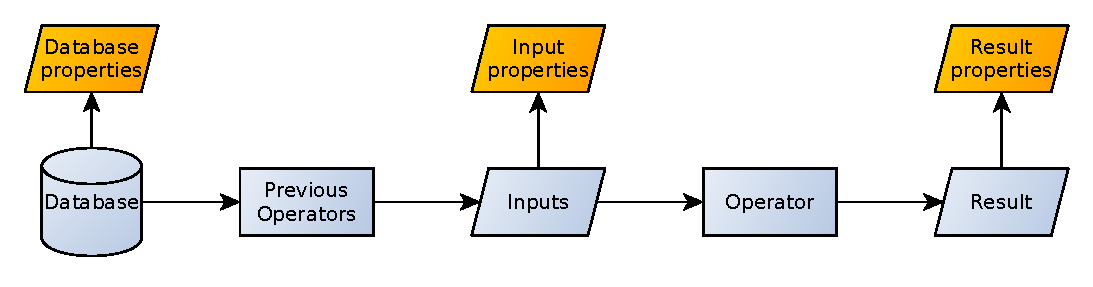
\includegraphics[width=0.9\textwidth]{figures/operator_properties_dependencies.pdf}
  \caption{Dependencies between operator inputs, result and logical
           properties.}
  \label{fig:op-dependencies}
\end{figure}

The estimated result properties can then be used as the input properties in the
next estimation step. The resulting chain of estimations is shown in
Figure \ref{fig:prop-estimation}.

\begin{figure}[h]
  \centering
  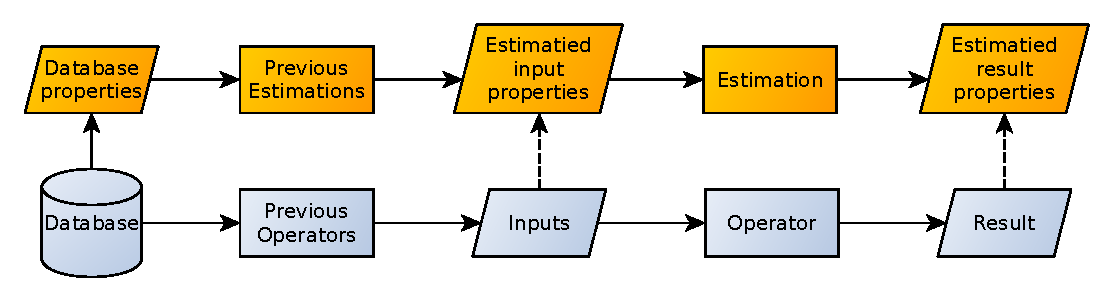
\includegraphics[width=0.9\textwidth]{figures/properties_estimation.pdf}
  \caption{Estimation of result properties.}
  \label{fig:prop-estimation}
\end{figure}


The more information we put into the logical properties, the more precise the
estimations will be. If the information is insufficient, the estimations can
diverge from the actual logical properties in a longer estimation chain
(symbolized by the dashed arrows in the above Figure).
However, storing more information also means increasing
memory consumption and processing time. This tradeoff has to be optimized.

In the following definitions, we formalize the idea that was just presented.

\begin{definition}[Estimation function]
  $\estfunc{o}$ is a logical properties estimation function of the operator
  $o \in \operators$ iff it has the following signature:\\
  
  \begin{samepage}
  \textbf{Input:}
  \begin{enumerate}
    \item $\props{G}$, the logical database properties.
    \item $\estprops{i_1}, \ldots, \estprops{i_n}$,
      the estimated logical properties of all inputs $i_1, \ldots, i_n$ of $o$.
  \end{enumerate}
  
  \textbf{Output:}\\
  
  $\estprops{o(i_1, \ldots, i_n)}$, an estimation of the logical properties of the
  output.
  \end{samepage}
\end{definition}

\begin{definition}[Estimated logical properties of an operator tree.]
  We define the estimated logical properties $\estprops{\Omega}$ of an
  operator tree $\Omega = o(i_1, \ldots, i_n)$ as
  \begin{displaymath}
    \estprops{\Omega}
      := \estfunc{o}(\props{G}, \estprops{i_1}, \ldots, \estprops{i_n})
  \end{displaymath}
\end{definition}

Now the logical properties of an operator tree can be estimated recursively as
shown in Figure \ref{fig:estimation-tree}.

\begin{figure}[ht]
 \begin{center}
   \begin{tikzpicture}
    \newcommand{\E}[1]{\estfunc{#1}}
    \small
    
    \node [block] (query) {
      $\estprops{\selection{h : \{ \text{Hobby} \}}(\expandout{x}{l : \{ \text{LIKES} \}}{h}(\selection{x : \{ \text{Person} \}}(\getnodes{x})))}$
    };
    
    \node [block] (hobby-label-selection) [below = of query] {$\E{\selection{h : \{ \text{Hobby} \}}}$};
    \node [block] (likes-expand) [below = of hobby-label-selection] {$\E{\expandout{x}{l : \{ \text{LIKES} \}}{h}}$};
    \node [block] (person-label-selection) [below = of likes-expand] {$\E{\selection{x : \{ \text{Person} \}}}$};
    \node [block] (get-nodes-as-x) [below = of person-label-selection] {$\E{\getnodes{x}}$};
    
    \draw[->] (likes-expand) edge node {} (hobby-label-selection);
    \draw[->] (person-label-selection) edge node {} (likes-expand);
    \draw[->] (get-nodes-as-x) edge node {} (person-label-selection);
    
    \node [block] at ([xshift=2cm]get-nodes-as-x.center) (db-props) {$\props{G}$};
    \draw[->] ([xshift=2cm]hobby-label-selection.center) -- (hobby-label-selection);
    \draw[->] ([xshift=2cm]likes-expand.center) -- (likes-expand);
    \draw[->] ([xshift=2cm]person-label-selection.center) --  (person-label-selection);
    \draw[->] (db-props) -- (get-nodes-as-x);
    \draw[-] (db-props) -- ([xshift=2cm]hobby-label-selection.center);
    
    \draw ([xshift=-0.5mm]hobby-label-selection.north) -- ([xshift=-0.5mm]query.south);
    \draw ([xshift=0.5mm]hobby-label-selection.north) -- ([xshift=0.5mm]query.south);
\end{tikzpicture}

 \end{center}
 \caption{Estimation graph for the logical properties of an operator tree.}
 \label{fig:estimation-tree}
\end{figure}

We will use these Definitions in our Neo4j implementation
(see Chapter \ref{chap:neo4j-impl}).
